
\section{Mathematical Background}%
\label{sec:mathematical_background}

We will in this section will we review standardized and well know methods and notations. Generally is the notation followed from \cite[Chapter 1]{pietro2012}.


\subsection{Notation}%
\label{sub:notation}

We will in this report assume $\Omega $ to be a compact and open set in $\mathbb{R} ^{d}$. Let $p \in \mathbb{R} $, $ 1 \le  p \le  \infty$, and  define the space $L^{p}\left( \Omega  \right) $ to be the set of all measurable functions $u: \Omega  \mapsto \mathbb{R} $ such that
$\left\lvert f \right\rvert ^{p}$ is Lebesgue integrable, i.e,

\begin{equation*}
    L^{p}\left( \Omega  \right) = \left\{ u: \Omega \mapsto \mathbb{R}  \mid \int_{\Omega }^{} \left\lvert u \right\rvert ^{p} d \Omega  < \infty  \right\}
.\end{equation*}
Let $u \in L^{p}\left( \Omega  \right) $. We define the integral norm of order $p$ to be \[
\| u \|_{ L^{p}\left( \Omega  \right)  }^{  }  = \left( \int_{\Omega }^{} \left\lvert u \right\rvert ^{p} dx  \right) ^{\frac{1}{p}}.
\]
Since $p=2$ is frequently used in this report, we also define for convenience a compact notation $\| u \|_{ \Omega  }^{  }  = \| u \|_{ L^{2}\left( \Omega  \right)  }^{  } $ .  Recall that $L^{2}\left( \Omega  \right) $ is a Hilbert space if it is equipped with a inner
product of two functions $u,v \in L^{2}\left( \Omega  \right) $ such that
    $
\left( u,v \right) _{\Omega } = \left( u,v \right) _{L^2\left( \Omega  \right) } = \int_{\Omega }^{} u  v dx.
$
The following definition for derivatives is employed,
\begin{equation}
\label{eq:mixed_derivative}
\partial ^{\alpha  } u = \frac{\partial ^{\left\lvert \alpha  \right\rvert } u}{ \partial ^{\alpha _{1} } x_{1} \partial ^{\alpha _{2}} x_{2}  }, \quad \text{for } \alpha=\left( \alpha _{1}, \alpha _{2} \right) \text{ and } f \in C^{\left\lvert \alpha  \right\rvert }
\left( \Omega  \right)
.\end{equation}
For $d$ dimensions of order $k$ we define the multi-index $\alpha  = ( \alpha _{1}, \ldots, \alpha _{d})  $ with the absolute value $\abs{ \alpha  } = \sum_{i=1}^{d}  \alpha _{i} = k $ s.t.
\[
\partial ^{\alpha} u = \frac{\partial ^{ \alpha_{1}  }  } {\partial^{} x_{1}^{\alpha _{1}}  } \ldots \frac{\partial ^{ \alpha_{d}  }  } {\partial^{} x_{d}^{\alpha _{d}}  } u
\]

  Let $m\ge 0$ be an integer and let $1 \le  p \le  \infty$ be a real number. Then the Sobolev space $H^{m}( \Omega ) $ are defined by
\[
H^{m}\left( \Omega  \right) = \left\{ u \in L^{2}\left( \Omega  \right)  \mid  \partial ^{\alpha } u \in L^{2}\left( \Omega  \right)  \forall \alpha : \left\lvert \alpha  \right\rvert  \le m \right\}.
\]
Equipped with the inner product for $u,v \in H^{m}\left( \Omega  \right) $, \[
    \left( u,v \right) _{H^{m}\left( \Omega   \right) } = \sum_{\left\lvert \alpha  \right\rvert  \le  m}^{}  \int_{\Omega }^{} \partial ^{\alpha } u \partial ^{\alpha } v dx,
\]
with the corresponding norm
$
\| u \|_{ H^{m}\left( \Omega  \right)  }^{2  }  =  \| u \|_{ L^{2}\left( \Omega  \right)    }^{2} + \sum_{k = 1}^{m}  \left\lvert u \right\rvert ^{2} _{  H^{k}\left( \Omega  \right) }.
$
Here the seminorm is defined such that, $ \left\lvert u \right\rvert _{H^{k}( \Omega  ) }^{2} =  \sum_{\left\lvert \alpha  \right\rvert  = k}^{} \| \partial ^{\alpha }u \|_{ \Omega  }^{ 2 }  .
$
We will often use the shorthand notation $ \| u \|_{ k, \Omega  }^{  } = \| u \|_{ H^{k}( \Omega)  }^{  } $ and $ \abs{ u }_{ k, \Omega  }^{  }  = \abs{ u }_{ H^{k}( \Omega)  }^{  }$.

Given the context of Sobolev spaces, we consider the functions $ u \in H^{2}( \Omega )$ and $ v \in H^{1}( \Omega )$. We can denote Greens theorem, which links integrals over a volume and its boundary, as follows,
\[
( \Delta u, v) _{\Omega } = -( \nabla u, \nabla v)_{\Omega } + ( u, \partial _{n}v)_{\Gamma }
\]
This identity serves as an essential tool for the calculations done.



\subsection{Computational Domains}%
\label{sub:computational_domain}
Assume that $\Omega \subset \mathbb{R} ^{d} $ is a compact set with a boundary  $\Gamma $. In standard FEM methods a key assumption is that the set $\Omega $ is a polyhedra. This is useful since a polyhedra can be fully covered by a collection of polyhedra and, hence, motivating us to define a fitted mesh.
We define a fitted mesh $\mathcal{T} $ of the domain $\Omega $ to be a collection of disjoint polyhedra $\left\{ T \right\}  $ forming a partition of $\Omega $ s.t $\overline{\Omega } = \bigcup _{T \in \mathcal{T} } T $, for illustration see Figure
\ref{fig:domain_mesh}.
Here we say that each $T \in  \mathcal{T} $ is a mesh element or an element.
The mesh size is defined as the maximum diameter $h := h_{max} $ of any polyhedra in the mesh $\mathcal{T} = \left\{ T \right\}  $, that is, $ h_{max} = \max_{T \in \mathcal{T} }  h_{T}$ s.t.
$h _{T}  = \mathrm{diam}\left( T \right)   = \mathrm{max}_{x_1, x_{2} \in T} \ \mathrm{ dist }(x_{1}, x_{2})$
Hence, motivating us to use the notation $\mathcal{T} _{h}$ for a mesh $\mathcal{T} $ with size $h$.

For simplicity will we restrict ourself to simplicial and quadrilateral elements.
A mesh $\mathcal{T}_{h}$ in $ \mathbb{R} ^{d}$ is said to be matching if
for all neighbouring elements $T_{1}, T_{2} \in \mathcal{T} _{h}$ such that the intersection $T_{1} \cap T_{2} $ is a manifold of dimensions $( d-1)$, then $T_{1} \cap T_{2} $ a entire facet of both $T_{1}$ and $T_{2}$.

Let the chunkiness parameter $c_{T} := h_{T}/r_{T}$, where $r_{T}$  is the largest ball that be inscribed inside a element $T \in \mathcal{T}_{h} $.
A mesh is said to be shape regular if $c_{T}\le  c$ is independent of $T$  and $h$. We also say that the mesh is quasi-uniform only if it is shape regular and $h_{\mathrm{ max }} \le  c h_{\mathrm{ min }}$.
For a more complete description of meshes, see \cite[Chapter 8]{ErnGuermond2021}.

In this thesis will we assume that a mesh $\mathcal{T}_{h} $ is matching, shape regular and quasi-uniform unless specified.
 The fact that the mesh is conform makes is a useful property since the interface between mesh elements has come into contact in the sense
that it is either a vertex or a facet. This with the combination of shape regularity and quasi-uniformity is a major key to prove important inequalities in broken Sobolev spaces \cite[Chapter 1.4.1]{pietro2012}. Hence, the assumptions are very handy when proving convergence.


Let $\mathcal{T}_{h}  = \left\{ T \right\} $ be a mesh of $\Omega \subset  \mathbb{R} ^d $ consisting of polygons $T \in \mathbb{R} ^{d}$.
The set of all facets is the union of external and internal facets, $\mathcal{F} _{h} = \mathcal{F} ^{ext}_{h} \cup \mathcal{F} _{h}^{int} $, where each are defined by
\[
            \mathcal{F}^{int} _{h}  = \left\{ F=T^{+}\cap T^{-}  \mid  T^{+}, T^{-} \in \mathcal{T}_{h}  \right\} \text{ and }
            \mathcal{F}^{ext} _{h}  = \left\{ F= \partial T \cap \partial \Omega    \mid  T  \in \mathcal{T}_{h}  \right\}.
\]
Assume $T^{+} \neq T^{-}$ . Next, we define the following normal vectors.
\begin{enumerate}[label=\arabic*)]
    \item We define $ n= n  _{\partial T}$ to be unit outward normal on $\partial T$ for each $T \in \mathcal{T}_{h} $
\item Let $F \in \mathcal{F }^{int} _{h}$. We define $n$ to be the facet normal $ n =  n _F = n | _{\partial T^{+}} $  from $T^{+}$ to $T^{-}$, illustrated in Figure \ref{fig:normal}. \red{Ask Andre about his comment here.}
 \item Let $F \in \mathcal{F} ^{ext}_{h}$. Then we define the facet normal $n | _{F} = n | _{\partial T} $ to be the unit outward normal.
\end{enumerate}
Please note that we for convenience employ the notation $n$ when it is clear what entity the normal is associated with.

    Let $v\in L^2( \Omega ) $ be a scalar function on $\Omega$ with a corresponding shape regular and quasi-uniform mesh $\mathcal{T}_{h} $. We will use the following definitions.
    \begin{enumerate}[label=\arabic*)]
        \item Let $F \in \mathcal{F}^{int} _{h}$ and $v^{\pm}| _{F} = \lim_{t\to 0^{+}} v( x \mp tn)   $ for $x \in F$. We define the mean as $\mean{ v} |_{F} = \frac{1}{2} (v^{+}_{F} + v^{-}_{F})   $ and the jump as $\jump{v}|_{F} =  v^{+}_{F} - v^{-}_{F} $.
        \item Let $F \in \mathcal{F}^{ext} _{h}$ and let $ v( x) =  v(x)|_{F} $ for  $x \in F$.
We define the mean as $\mean{ v} |_{F} = v    $ and the jump as $\jump{v}|_{F} = v$.

    \end{enumerate}
    To simplify will we use the notation $\mean{ v } = \mean{ v }|_{F}    $ and $\jump{ v } = \jump{ v }| _{F}    $ for all $F \in \mathcal{F} _{h}$.
    Remark that if we have two functions $u,v$, for which $u^{\pm}( x) $ and $v^{\pm}( x) $ are defined, then the following identity holds $  \jump{ uv }    = \jump{ u }   \mean{ v }    + \mean{ u }  \jump{ v }$ along all facets $ \mathcal{F}_{h} $ associated with the
    triangulation $\mathcal{T} _{h}$.


\begin{figure}[h!]
\centering
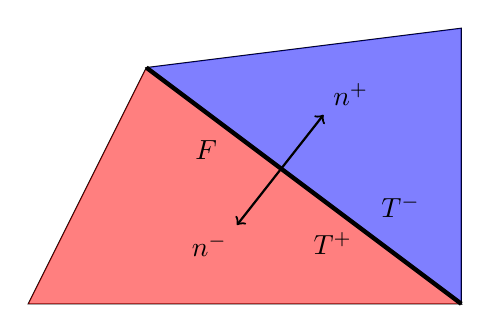
\begin{tikzpicture}[scale=1]
\coordinate (A) at (-1.5, -0);
\coordinate (C) at (0,3);
\coordinate (B) at (4,0);
\coordinate (D) at (4,3.5);

\draw (A) -- (B) -- (C) -- cycle;
\draw (B) -- (C) -- (D) -- cycle;
\fill[red, opacity=0.5] (A) -- (B) -- (C);
\fill[blue, opacity=0.5] (B) -- (C) -- (D);
\draw[ultra  thick] (C) -- (B);

\coordinate (Tm) at (3.6,1.5);
\coordinate (Tp) at (2.0, 0.5);
\coordinate (e) at (0.5, 2.2);
\node[below left] at (Tm) {$T^{-} $ };
\node[above right] at (Tp) {$T^{+}$ };
\node[below right] at (e) {$F$ };

\coordinate (start) at (1.7, 1.7);
\coordinate (endPlus) at (2.25, 2.4);
\coordinate (endMinus) at (1.15, 1.0);

\draw [->, thick] (start) -- (endPlus);
\node[above right] at (endPlus) {$n^{+}$};

\draw [->, thick] (start) -- (endMinus);
\node[below left] at (endMinus) {$n^{-}$};

\end{tikzpicture}

\caption{Facet $F \in \mathcal{F}_h^{int} $ shared by the triangles $T^{+}, T^{-} \in \mathcal{T}_{h} $ and the normal unit vector $n^{+}$ and $n^{-}$. If we pick $T=T^{+}$ and want to evaluate the normal vector $n$ along a facet $F$, then we define $n = n  \mid _{F} = n^{+}$.}
    \label{fig:normal}
\end{figure}



\subsection{Broken Sobolev spaces}%
\label{sub:broken_sobolev_spaces}

In this work will we compute norms on discontinuous elements, thus, it will be necessary to define broken Sobolev spaces.
Let $\mathcal{T}_{h} $ be a mesh and some integer $m\le n$. Then we define the broken Sobolev space to be \[
    \begin{split}
H^{m}( \mathcal{T}_{h} ) & := \left\{ v \in L^2( \Omega )  \mid \ v|_{T} \in H^{m}( T) \quad     \forall T \in  \mathcal{T} \right\}\\
        L^{2}( \mathcal{F}_{h} ) &:= \left\{ v \in L^2( \mathcal{T}_{h}  )  \mid   \ v|_{F} \in L^{2}( F)  \quad  \forall F \in  \mathcal{F}_{h}   \right\}.
    \end{split}
\]
This motivates us to define broken Sobolev norms and inner products using summation over mesh elements,
\[
 \| v \|_{H^{m}( \mathcal{T}_{h} ) }^{2} = \sum_{T \in  \mathcal{T}_{h} }^{} \| v  \|_{ H^{m}( T ) }^{2  } \quad \text{ and } \quad
 (v ,w )_{H^{m}( \mathcal{T}_{h} ) }^{} = \sum_{T \in \mathcal{T} _{h}}^{} (v ,w )_{ H^{m}( T ) }^{  } .
\]
As before, we use the shorthand notation,  $\| v \|_{\mathcal{T}_{h}} =  \| v \|_{L^{2}( \mathcal{T}_{h} ) }$ and  $(v ,w )_{ \mathcal{T}_{h} }^{} = (v ,w )_{L^2( \mathcal{T}_{h} ) }^{} $.
That is,
\[
 \| v \|_{L^{2}( \mathcal{F}_{h} ) }^{2} = \sum_{F \in  \mathcal{F}_{h} }^{} \| v  \|_{ L^{2}( F ) }^{2  } \quad \text{ and } \quad
 (v ,w )_{L^{2}( \mathcal{F}_{h} ) }^{} = \sum_{T \in \mathcal{F} _{h}}^{} (v ,w )_{ L^{2}( F ) }^{  } .
\]
Again, we often use the more compact notation $\| v \|_{\mathcal{F}_{h}} =  \| v \|_{L^{2}( \mathcal{F}_{h} ) }$ and  $(v ,w )_{ \mathcal{F}_{h} }^{} = (v ,w )_{L^2( \mathcal{F}_{h} ) }^{} $.
A very useful lemma when working with estimates on broken Sobolev spaces is that a if a function is continuous, then the jump between the mesh elements is zero. A function $ v \in  H^{1}( \mathcal{T}_{h} ) $ belongs to $ H^{1}( \Omega )  $ if and only
if $ \jump{ v }   = 0 \text{ for }  F \in \mathcal{F}^{int}_{h}$.



\subsection{Useful inverse estimates}%
\label{sub:useful_inverse_estimates}

We first some the standard inequalities.
\begin{enumerate}[label=(\roman*)]
    \item A fundamental property of the inner-product the so-called Cauchy-Schwarz inequality
    \[
     ( u,v)_{H^{m}( \Omega )  }   \le \| u \|_{H^{m}( \Omega )   }^{  } \| v \|_{H^{m}( \Omega )    }^{  } \forall u,v \in H^{m}( \Omega )
    \]

    \item For any $a,b >\mathbb{R} $ the well known Youngs $\varepsilon $-inequality is on the form,
        \[
            2ab \le \varepsilon a^2+ \frac{1}{\varepsilon } b^2.
        \]
\end{enumerate}

Choose any triangle $T \in \mathcal{T}_{h} $ and let $v \in \mathcal{P}( T)  $. Then does the local inverse estimate hold,
$$
\abs{ v }_{H^{l}( T) } \lesssim h^{m-l} \abs{ v }_{H^{m}( \Omega ) }.
$$
for $l \le m$. For proof, see \cite[Lemma 12.1]{ErnGuermond2021}. An essential example is the following inequality.
$$\| D^2v \|_{T  }^{ 2 } \lesssim h^{-1} \| \nabla v  \|_{ T  }^{  } \lesssim h^{-2} \| v \|_{T  }^{  }   $$

Another very useful inequality is the so-called trace inequality which connect the relationship of evaluating the norm on element $ T $ and with any of the corresponding facets $F \in \partial T$. The general form is $\| v \|_{F   }^{  }  \lesssim
h^{-\frac{1}{2}} \| v \|_{ T  }^{  } $, see \cite[Lemma 12.8]{ErnGuermond2021}.
Let $\partial _{n} v = \nabla v \ n$ and $\partial_{nn} v = n^{T} D^2 v \ n $, and keeping in mind that the normal vector has a unit length, can we evidently apply the trace inverse inequality to conclude, \[
\begin{split}
    \| \partial _{n} v \|_{F  }^{  }  & \le \| \nabla v \|_{F  }^{  }  \le h^{-\frac{1}{2}} \| \nabla  v \|_{T  }^{  },  \\
    \| \partial _{nn} v \|_{ F }^{  } & \le  \| D^2 v \|_{ F }^{  }   \le  h^{-\frac{1}{2}} \| D^2 v \|_{ T }^{  }.
\end{split}
\]

% \begin{enumerate}[label=(\roman*)]
%     \item General inverse inequality.
%     Let $\alpha = ( \alpha _{1}, \ldots, \alpha _{N}) $ and $\beta = ( \beta _{1}, \ldots, \beta _{N} ) $.
%     Assume $u \in H^{\abs{ \beta  }  }( T) $. The following inverse inequalities hold.
%     \[
%         \begin{split}
%         \| \partial ^{\alpha } u \|_{T  }^{  } & \lesssim h^{ - \abs{ \beta  }  } \| \partial ^{\alpha - \beta } u \|_{T }^{  } \\
%         \| \partial ^{\alpha }_{n} u  \|_{F  }^{  } &\lesssim h^{-\frac{1}{2}  } \| \partial ^{\alpha } u \|_{T }^{  }
%         \end{split}
%     \]
% \end{enumerate}
    % For a full triangle we have \[
    % \| v \|_{ \partial T }^{  } \lesssim h_{T}^{-\frac{1}{2}} \| v \|_{ T }^{  } + h_{T}^{\frac{1}{2}} \| \nabla v \|_{ T }^{  }
    % \]




\subsection{Lax-Milgram lemma}%
\label{sub:lax_milgram_lemma}

The intention is to introduce a abstract framework which can handle various types of partial differential equations (PDE). Let  $\mathcal{A} : X \to Y $ be a abstract linear operator encoding the structure of any linear PDE, including boundary
conditions and $X,Y$ are spaces of functions. Then we denote the abstract strong formulation as the equation
\begin{equation}
\label{eq:strong_abs}
\mathcal{A} u = f.
\end{equation}
What we will see is that Sobolev spaces are designed to study this kinds of problems.


\begin{definition}[Linear bounded functional]
    \label{def:linear_function}
Let $X$ be a Hilbert space. Furthermore, we define the dual space $X' $ to be the space of linear and bounded functionals $F: X  \mapsto \mathbb{R} $, i.e., \[
X'  = \left\{ F: X \to \mathbb{R}   \mid  F \text{ is linear and bounded} \right\}
\]
\end{definition}

\begin{problem}[Abstract linear problem]
    \label{def:abstract_linear_problem}
    Assume $X$ and $Y$  to be two Hilbert spaces. Let the vector space $\mathcal{L}( X,Y)  $ be all linear bounded operators spanned from $X$ to $Y$. We define the abstract linear problem as follows; find $u \in X$ s.t. \[
    a( u,v)  = l(v ) := \left<f,v \right>_{X' , X}  \forall v \in X
    \]
    Where $a \in  \mathcal{L} ( X, X,\mathbb{R} ) $ is a bounded bilinear form and $f \in X':= \mathcal{L} ( X,\mathbb{R} )  $ is a bounded linear form associated with the abstract strong formulation \eqref{eq:strong_abs}. Here we denote by $\left<\cdot ,\cdot  \right>_{X' .X} $ the duality pairing between $X' $ and $X
    $.

\end{problem}


\begin{definition}[Coercivity and Boundedness]
    \label{def:coercivity}
    Let $X$ be a Hilbert space and let $a( \cdot ,\cdot )  \in  \mathcal{L} ( X, X,\mathbb{R} )  $. Recall that the bilinear form $a( \cdot ,\cdot ) $ is coercive on $X$ if there exists an constant $C_{1} > 0 $ such that \[
     a( v,v) \ge  C_{2} \| v \|_{ X }^{  } \quad  \forall v \in  X
    \]
     The bilinear form $a( \cdot ,\cdot ) $ is said to bounded if there exists an constant $C_{2}$  \[
    a( u,v)  \le C_{1} \| u \|_{ X }^{  }  \| v \|_{X }^{  }
    \]
\end{definition}


\begin{lemma}[Lax-Milgram]
    \label{def:lax-milgram}
    The abstract linear problem \ref{def:abstract_linear_problem} is well-posed if $a(\cdot , \cdot  ) $ is bounded and coercive. Moreover, the following a priori estimate holds true.\[
    \| v \|_{ X }^{  } \lesssim  \| f \|_{ X'  }^{  }
    \]
\end{lemma}
\begin{proof}
    The problem can easily be proved using a special case of the Banach–Nečas–Babuška theorem. See \cite[Lemma 1.4]{pietro2012}
\end{proof}



\subsection{Finite element method}%
\label{sub:finite_element_method}


The finite element method (FEM) is a numerical method to solve partial differential equation by finding an approximation of the Problem \ref{def:abstract_linear_problem}.  Let $X_{h}$ be a finite-dimensional (polynomial) approximation space on the mesh
$\mathcal{T} _{h}$. We say that a method is conform if $X_{h}\subset X $ and non-conform if $X _{h} \not\subset X$. We define the approximate problem as follows.
\begin{problem}[The approximate problem]
    \label{def:approx_problem}
    Find  $u_{h} \in X_{h}$ s.t. \[
    a_{h}(u_{h},v ) = l_{h}( v) :=  \left<f,v \right>   \forall v \in X_{h}
    \]
\end{problem}

We denote the functional $a_{h}: X_{h} \times X_{h} \to \mathbb{R} $ as an consistent approximation of $a: X \times X \to \mathbb{R} $, and similarly for the right-hand side $l_{h} : \times _{h} \to \mathbb{R} $ as an approximation of $l: X \to \mathbb{R} $.
In this report will we generally specify any discrete space $X_{h}(\mathcal{T}_{h})$  as the $C^{0}$ continuous polynomial space $\mathcal{P}^{k}(\mathcal{T}_{h})$, of order $k$.

\begin{definition}[Broken polynomial spaces]
    Let $\mathcal{T}_{h} $ be a mesh of $\Omega \in \mathbb{R} ^{d} $. Let $\mathcal{P}^{k}(T) $ be the space of all polynomials of order $k$ in the mesh element $T$ in $\mathcal{T}_{h}$ . We define the broken polynomial space as \[
    \mathcal{P}^{k} ( \mathcal{T}_{h} ) := \left\{ v \in L^{2}( \mathcal{T}_{h} )    \mid  v|_{T} \in \mathcal{P}^k( T) \quad  \forall T \in  \mathcal{T}_{h}   \right\}.
    \]
    Similarly, the global $C^{0}$ continuous polynomial space is denoted as
    \[
    \mathcal{P}^{k}_{c} ( \mathcal{T}_{h} ) := \left\{ v \in C^{0}( \Omega )   \mid  v|_{T} \in \mathcal{P}^k( T) \quad  \forall T \in  \mathcal{T}_{h}   \right\}.
    \]

\end{definition}



\begin{definition}[Local polynomial space]
    \label{def:local_space}
    Let $T$ be a element in a mesh $\mathcal{T}_{h} $,  $x = \left[ x_{1}, \ldots, x_{d} \right] $ be a vector, and $\alpha  = \left[ \alpha _{1}, \ldots, \alpha _{d} \right] \in \mathbb{N} ^{d} $ be a multi index.
    The local polynomial space $\mathcal{P} ^{k}( T) $ for a simplex is denoted as
    \begin{equation}
    \label{eq:pol_space}
        \mathcal{P}^{k}( T) =  \mathrm{span}\left\{ x^{\alpha } \ \text{for } x \in T \text{ and } 0 \le  \alpha _{i} \le k \right\}.
    \end{equation}
    where  $x^{\alpha }$ is a monomial such that $x^{\alpha } = x_{1}^{\alpha _{1}} \ldots x_{d}^{\alpha _{d}}$.

    Let $T$ be a cuboid, i.e.,  $T = \prod_{i=1}^{d} [z_{i}^{-},z_{i}^{+}]$ where $z_{i}^{-}< z_{i}^{+}$ for $z_{i}^{\pm} \in \mathbb{R} $. Then the polynomial space $\mathcal{Q}^{k}( T)$  in $\mathbb{R} ^{d}$ is defined as the tensor product of 1-dimensional
    finite elements, i.e.,
      \[
    \mathcal{Q} _{k}(T)  := \mathcal{P}^{k}( [z_{1}^{-},z_{1}^{+}] ) \otimes \ldots \otimes \mathcal{P}^{k}( [z_{d}^{-},z_{d}^{+}] )
    \]
\end{definition}
For more information about the local polynomial spaces, see \cite[Chapter 6.4, 7.3]{ErnGuermond2021}

Following Ciarlet \cite[pp.93]{ciarlet1991basic}, the abstract definition of a finite element is defined as the triplet $( T, \mathcal{P}, \Sigma ) $. In our case is $T$ a simplex or a quadrilateral geometry and the $\mathcal{P} $ a finite dimensional polynomial space consisting of $N$ shape
functions $\left\{ \phi_{i}  \right\}_{i\in N} $ such as \eqref{eq:pol_space}.
On the other hand, $\Sigma $ is the so-called dual of $\mathcal{P}$, that is, the set of linear forms $\left\{ \sigma _{i} \right\} $ such that. $ \sigma_{j} ( \phi_{i} ) = \delta _{ij}$ and $p( x) = \sum_{i\in N}^{} \sigma_{i} ( p) p_{i} $.
If there is a set of points $\left\{ a_{i} \right\}_{i \in N} $  in $T$ such that
$\sigma_{i}( p) = p( a_{i}) \  \forall p \in \mathcal{P}$,  then the triple $( T, \mathcal{P}, \Sigma  ) $ is called a Lagrangian finite element. The set of points $\left\{ a_{i} \right\}_{i \in N}  $ is called nodes and is associated with the
so-called nodal basis of $\mathcal{P} $ such that  $\phi ( a_{i}) = \delta _{ij} \ \forall i,j  \in N$

As anticipated, the local node configuration of the polynomial space, denoted as $\mathcal{P}^{k}( T)$, is influenced by the form of $T$. For the purpose of our discussion, let us represent the polynomial basis for a simplicial element and a quadrilateral
element as $\mathcal{P} ^{k}(T )$ and $\mathcal{Q} ^{k}( T)$, both of polynomial order $k$. In Figure \ref{fig:ill_nodes} is it illustrated for  $k=1,2,3$ in dimension $d=2$ on how the node configuration evolve.

\begin{figure}[h!]
    \centering
    \hfill
    \subfloat[$\mathcal{P}^{1}( T)  $]{
        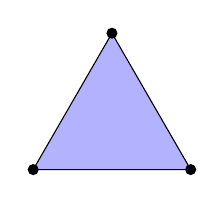
\begin{tikzpicture}[scale=1.0]
            % Define the coordinates
            \coordinate (A) at (0,0);
            \coordinate (B) at (2,0);
            \coordinate (C) at (1,{sqrt(3)});

            % Draw the triangle
            \fill[blue!30] (A) -- (B) -- (C) -- cycle;
            \draw (A) -- (B) -- (C) -- cycle;

            % Draw the nodes
            \fill (A) circle (2pt);
            \fill (B) circle (2pt);
            \fill (C) circle (2pt);
        \end{tikzpicture}
    }
    \hfill
    \subfloat[ $\mathcal{P}^{2}( T)  $]{
        \begin{tikzpicture}[scale=1.0]
            % Define the coordinates
            \coordinate (A) at (0,0);
            \coordinate (B) at (2,0);
            \coordinate (C) at (1,{sqrt(3)});

            % Define the midpoints
            \coordinate (D) at ($(A)!0.5!(B)$);
            \coordinate (E) at ($(B)!0.5!(C)$);
            \coordinate (F) at ($(A)!0.5!(C)$);

            % Draw the triangle
            \fill[blue!30] (A) -- (B) -- (C) -- cycle;
            \draw (A) -- (B) -- (C) -- cycle;

            % Draw the nodes
            \fill (A) circle (2pt);
            \fill (B) circle (2pt);
            \fill (C) circle (2pt);
            \fill (D) circle (2pt);
            \fill (E) circle (2pt);
            \fill (F) circle (2pt);
        \end{tikzpicture}
    }
    \hfill
    \subfloat[$\mathcal{P} ^{3}( T)  $ ]{
        \begin{tikzpicture}[scale=1.0]
            % Define the coordinates
            \coordinate (A) at (0,0);
            \coordinate (B) at (2,0);
            \coordinate (C) at (1,{sqrt(3)});

            % Define the additional points along the edges
            \coordinate (D) at ($(A)!0.3333!(B)$);
            \coordinate (E) at ($(B)!0.3333!(C)$);
            \coordinate (F) at ($(C)!0.3333!(A)$);
            \coordinate (G) at ($(A)!0.6667!(B)$);
            \coordinate (H) at ($(B)!0.6667!(C)$);
            \coordinate (I) at ($(C)!0.6667!(A)$);

            % Define the centroid
            \coordinate (J) at (1, {sqrt(3)/3});

            % Draw the triangle
            \fill[blue!30] (A) -- (B) -- (C) -- cycle;
            \draw (A) -- (B) -- (C) -- cycle;

            % Draw the nodes
            \fill (A) circle (2pt);
            \fill (B) circle (2pt);
            \fill (C) circle (2pt);
            \fill (D) circle (2pt);
            \fill (E) circle (2pt);
            \fill (F) circle (2pt);
            \fill (G) circle (2pt);
            \fill (H) circle (2pt);
            \fill (I) circle (2pt);
            \fill (J) circle (2pt);
        \end{tikzpicture}
    }
    \\
    \hfill
    \subfloat[$\mathcal{Q}^{1}( T)  $]{
        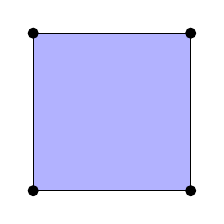
\begin{tikzpicture}[scale=1.0]
            % Define the coordinates
            \coordinate (A) at (0,0);
            \coordinate (B) at (2,0);
            \coordinate (C) at (2,2);
            \coordinate (D) at (0,2);

            % Draw the square
            \fill[blue!30] (A) -- (B) -- (C) -- (D) -- cycle;
            \draw (A) -- (B) -- (C) -- (D) -- cycle;

            % Draw the nodes
            \fill (A) circle (2pt);
            \fill (B) circle (2pt);
            \fill (C) circle (2pt);
            \fill (D) circle (2pt);
        \end{tikzpicture}
    }
    \hfill
    \subfloat[ $\mathcal{Q} ^{2}( T)  $]{
        \begin{tikzpicture}[scale=1.0]
            % Define the coordinates
            \coordinate (A) at (0,0);
            \coordinate (B) at (2,0);
            \coordinate (C) at (2,2);
            \coordinate (D) at (0,2);

            % Define the midpoints
            \coordinate (E) at ($(A)!0.5!(B)$);
            \coordinate (F) at ($(B)!0.5!(C)$);
            \coordinate (G) at ($(C)!0.5!(D)$);
            \coordinate (H) at ($(D)!0.5!(A)$);
            % Define the centroid
            \coordinate (M) at (1, 1);

            % Draw the square
            \fill[blue!30] (A) -- (B) -- (C) -- (D) -- cycle;
            \draw (A) -- (B) -- (C) -- (D) -- cycle;

            % Draw the nodes
            \fill (A) circle (2pt);
            \fill (B) circle (2pt);
            \fill (C) circle (2pt);
            \fill (D) circle (2pt);
            \fill (E) circle (2pt);
            \fill (F) circle (2pt);
            \fill (G) circle (2pt);
            \fill (H) circle (2pt);
            \fill (M) circle (2pt);
        \end{tikzpicture}
    }
    % And so on for $\mathcal{P}^{3}( S)  $, $\mathcal{P}^{4}( S)  $, etc.
    \hfill
    \subfloat[ $\mathcal{Q} _{3}( T)  $]{
        \begin{tikzpicture}[scale=1.0]
            % Define the coordinates
            \coordinate (A) at (0,0);
            \coordinate (B) at (2,0);
            \coordinate (C) at (2,2);
            \coordinate (D) at (0,2);

            % Define the additional points along the edges
            \coordinate (E) at ($(A)!0.3333!(B)$);
            \coordinate (F) at ($(B)!0.3333!(C)$);
            \coordinate (G) at ($(C)!0.3333!(D)$);
            \coordinate (H) at ($(D)!0.3333!(A)$);
            \coordinate (I) at ($(A)!0.6667!(B)$);
            \coordinate (J) at ($(B)!0.6667!(C)$);
            \coordinate (K) at ($(C)!0.6667!(D)$);
            \coordinate (L) at ($(D)!0.6667!(A)$);

            % Define the internal nodes
            \coordinate (M) at ($(E)+(0,0.6667)$);
            \coordinate (N) at ($(E)+(0,1.332)$);
            \coordinate (O) at ($(I)+(0,0.6667)$);
            \coordinate (P) at ($(I)+(0,1.332)$);

            % Draw the square
            \fill[blue!30] (A) -- (B) -- (C) -- (D) -- cycle;
            \draw (A) -- (B) -- (C) -- (D) -- cycle;

            % Draw the nodes
            \fill (A) circle (2pt);
            \fill (B) circle (2pt);
            \fill (C) circle (2pt);
            \fill (D) circle (2pt);
            \fill (E) circle (2pt);
            \fill (F) circle (2pt);
            \fill (G) circle (2pt);
            \fill (H) circle (2pt);
            \fill (I) circle (2pt);
            \fill (J) circle (2pt);
            \fill (K) circle (2pt);
            \fill (L) circle (2pt);
            \fill (M) circle (2pt);
            \fill (N) circle (2pt);
            \fill (O) circle (2pt);
            \fill (P) circle (2pt);
        \end{tikzpicture}
        }
        \caption{Illustration of the nodes for the element of a simplex a quadrilateral for dimension $d=2$ for polynomial orders $k=1,2,3$.}
        \label{fig:ill_nodes}
\end{figure}


We may introduce the reference element $\hat{T} $ in $d$ dimensions. The reference for a quadrilateral is denoted as $\hat{T} = [0,1]^{d}$. The reference for a simplex in  is defined by the convex hull spanned by the points $( z_{0}, e_{1}, \ldots, e_{d}) $ where $z_{0}:=0$ is the origin and $ \left\{ e_{i}
\right\}_{i=1}^{d} $ is the standard Cartesian  unit basis in $ \mathbb{R} ^{d} $. A corresponding reference finite element is defined as $( \hat{T}, \hat{\mathcal{P} }, \hat{\Sigma}   ) $.



\begin{figure}[th!]
    \centering
    \hspace{-2.2cm}  % Adjust the space as necessary
    \subfloat[]{
        \begin{tikzpicture}[scale=1.0]
            % Define the Reference triange
            \coordinate (A) at (0,0);
            \coordinate (B) at (1,0);
            \coordinate (C) at (0,1);
            \coordinate (G1) at (1/3,1/3);

            \fill[red!30] (A) -- (B) -- (C) -- cycle;
            \draw (A) -- (B) -- (C) -- cycle;
            \fill (A) circle (2pt);
            \fill (B) circle (2pt);
            \fill (C) circle (2pt);

            % Define the arbitary triange
            \coordinate (D) at (2,0);
            \coordinate (E) at (4,0);
            \coordinate (F) at (3,{sqrt(2)});
            \coordinate (G2) at (3, {sqrt(3)/3});

            \fill[blue!30] (D) -- (E) -- (F) -- cycle;
            \draw (D) -- (E) -- (F) -- cycle;
            \fill (D) circle (2pt);
            \fill (E) circle (2pt);
            \fill (F) circle (2pt);

            % Draw arrow to signify the mapping G
            \draw[->, thick, >=stealth] ($(G1)+(0.2,0.2)$) to[bend left] node[midway, above, yshift=0.1cm] {$\mathcal{G}$} ($(G2)+(-0.2,0.2)$);
        \end{tikzpicture}
    }
    \hspace{2.0cm}  % Adjust the space as necessary
    \subfloat[]{
        \begin{tikzpicture}[scale=1.0]
            % Define the Reference quadrilateral
            \coordinate (A) at (0,0);
            \coordinate (B) at (1,0);
            \coordinate (C) at (1,1);
            \coordinate (D) at (0,1);
            \coordinate (G1) at (0.5,0.5);

            \fill[red!30] (A) -- (B) -- (C) -- (D) -- cycle;
            \draw (A) -- (B) -- (C) -- (D) -- cycle;
            \fill (A) circle (2pt);
            \fill (B) circle (2pt);
            \fill (C) circle (2pt);
            \fill (D) circle (2pt);

            % Define the arbitrary quadrilateral
            \coordinate (E) at (2,0);
            \coordinate (F) at (3,1);
            \coordinate (G) at (3,2);
            \coordinate (H) at (2,1);
            \coordinate (G2) at (2.5,0.5);

            \fill[blue!30] (E) -- (F) -- (G) -- (H) -- cycle;
            \draw (E) -- (F) -- (G) -- (H) -- cycle;
            \fill (E) circle (2pt);
            \fill (F) circle (2pt);
            \fill (G) circle (2pt);
            \fill (H) circle (2pt);

            % Draw arrow to signify the mapping G
            \draw[->, thick, >=stealth] ($(G1)+(0.3,0.1)$) to[bend left] node[midway, above, yshift=0.1cm] {$\mathcal{G}$} ($(G2)+(-0.2,0.2)$);
        \end{tikzpicture}
    }
    \\
    \subfloat[]{
        \begin{tikzpicture}[scale=1.0]
            % Define the Reference tetra
            \coordinate (A) at (0,0);
            \coordinate (B) at (1,0);
            \coordinate (C) at (0,1);
            \coordinate (D) at (0.7,0.7);
            \coordinate (G1) at (1/3,1/3);

            \fill[red!65] (A) -- (B) -- (C) -- cycle;
            \fill[red!30] (D) -- (B) -- (C) -- cycle;
            \draw (A) -- (B) -- (C) -- cycle;
            \draw (D) -- (B) -- (C) -- cycle;
            \draw[dashed] (A) -- (D);
            \fill (A) circle (2pt);
            \fill (B) circle (2pt);
            \fill (C) circle (2pt);
            \fill (D) circle (2pt);


            % Define the Translated tetra
            \coordinate (A') at ($(A) + (2,0)$);
            \coordinate (B') at ($(B) + (2,0)$);
            \coordinate (C') at ($(C) + (2.6, 0.6)$);
            \coordinate (D') at ($(D) + (2.5, 0.2)$);

            \fill[blue!65] (A') -- (B') -- (C') -- cycle;
            \fill[blue!30] (D') -- (B') -- (C') -- cycle;
            \draw (A') -- (B') -- (C') -- cycle;
            \draw (D') -- (B') -- (C') -- cycle;
            \draw[dashed] (A') -- (D');
            \fill (A') circle (2pt);
            \fill (B') circle (2pt);
            \fill (C') circle (2pt);
            \fill (D') circle (2pt);

            % Draw arrow to signify the mapping G
            \draw[->, thick, >=stealth] ($(G1)+(0.6,0.2)$) to[bend left] node[midway, above, yshift=0.1cm] {$\mathcal{G}$} ($(D')+(-0.6,0.1)$);
        \end{tikzpicture}
    }
    \hspace{2cm}  % Adjust the space as necessary
    \subfloat[]{
        \begin{tikzpicture}[scale=1.0]
    % Define the Reference cube
    \coordinate (A) at (0,0);
    \coordinate (B) at (1,0);
    \coordinate (C) at (1,1);
    \coordinate (D) at (0,1);
    \coordinate (E) at (0.3,0.3);
    \coordinate (F) at (1.3,0.3);
    \coordinate (G) at (1.3,1.3);
    \coordinate (H) at (0.3,1.3);

    \fill[red!65] (A) -- (B) -- (C) -- (D) -- cycle;
    \fill[red!45] (D) -- (H) -- (G) -- (C) -- cycle;
    \fill[red!30] (B) -- (C) -- (G) -- (F) -- cycle;
    \draw (A) -- (B) -- (C) -- (D) -- cycle;
    \draw (A) -- (E) -- (F) -- (B);
    \draw (D) -- (H) -- (G) -- (C);
    \draw[dashed] (E) -- (H);
    \draw[dashed] (F) -- (G);

    % Define the Translated cube
    \coordinate (A') at ($(A) + (3.3, 0.0)$);
    \coordinate (B') at ($(B) + (3.3, 0.0)$);
    \coordinate (C') at ($(C) + (3.3, 0.0)$);
    \coordinate (D') at ($(D) + (3.3, 0.0)$);
    \coordinate (E') at ($(E) + (2.2, 0.3)$);
    \coordinate (F') at ($(F) + (2.2, 0.3)$);
    \coordinate (G') at ($(G) + (2.2, 0.3)$);
    \coordinate (H') at ($(H) + (2.2, 0.3)$);

    \fill[blue!65] (A') -- (B') -- (C') -- (D') -- cycle;
    \fill[blue!30] (D') -- (H') -- (G') -- (C') -- cycle;
    \fill[blue!45] (D') -- (A') -- (E') -- (H') -- cycle;
    \draw (A') -- (B') -- (C') -- (D') -- cycle;
    \draw (A') -- (E') -- (F') -- (B');
    \draw (D') -- (H') -- (G') -- (C');
    \draw[dashed] (E') -- (H');
    \draw[dashed] (F') -- (G');

    % Draw arrow to signify the mapping G
    \draw[->, thick, >=stealth] ($(A)+(0.8,0.5)$) to[bend left] node[midway, above, yshift=0.1cm] {$\mathcal{G}$} ($(A')+(-0.5,0.8)$);
\end{tikzpicture}
    }
    \caption{Illustration of affine mapping $\mathcal{G} : \hat{T} \to T $ in dimensions $d=2,3$ from a reference element $\hat{T}$  to element $T$ for simplexes and and quadrilaterals.  } \label{fig:affine_mapping}
\end{figure}

Let the mapping $\mathcal{G} : \hat{T} \to  T$ as the affine
mapping, i.e. $\mathcal{G}(x) = Ax +
b$.
The important property of affine transformations is the preservation of parallelism. This means that for any two vectors $x,y \in  \hat{T}$ that are parallel in the reference triange, then their images $\mathcal{G}(x)  $  and $\mathcal{G}( y)  $ will
also be parallel. Generally speaking, an affine transformation of the reference simplex is a transformation to any another simplex of the same dimension. However, for any quadrilateral, an affine transformation preserves the parallelism of opposite
sides, for an illustration see Figure \ref{fig:affine_mapping} and for a counter example see Figure \ref{fig:nonaffine}.

\begin{figure}[h!]
    \centering
    \hspace{-2.2cm}  % Adjust the space as necessary
    \subfloat[]{
        \begin{tikzpicture}[scale=1.0]
            % Define the Reference quadrilateral
            \coordinate (A) at (0,0);
            \coordinate (B) at (1,0);
            \coordinate (C) at (1,1);
            \coordinate (D) at (0,1);
            \coordinate (G1) at (0.5,0.5);

            \fill[red!30] (A) -- (B) -- (C) -- (D) -- cycle;
            \draw (A) -- (B) -- (C) -- (D) -- cycle;
            \fill (A) circle (2pt);
            \fill (B) circle (2pt);
            \fill (C) circle (2pt);
            \fill (D) circle (2pt);

            % Define the arbitrary quadrilateral
            \coordinate (E) at (2,0);
            \coordinate (F) at (3,0);
            \coordinate (G) at (3.5,1);
            \coordinate (H) at (2.5,1);
            \coordinate (G2) at (2.5,0.5);

            \fill[blue!30] (E) -- (F) -- (G) -- (H) -- cycle;
            \draw (E) -- (F) -- (G) -- (H) -- cycle;
            \fill (E) circle (2pt);
            \fill (F) circle (2pt);
            \fill (G) circle (2pt);
            \fill (H) circle (2pt);

            % Draw arrow to signify the mapping G
            \draw[->, thick, >=stealth] ($(G1)+(0.3,0.1)$) to[bend left] node[midway, above, yshift=0.1cm] {$\mathcal{G}$} ($(G2)+(-0.2,0.2)$);
        \end{tikzpicture}
    }
    \hspace{2.0cm}  % Adjust the space as necessary
    \subfloat[]{
        \begin{tikzpicture}[scale=1.0]
            % Define the Reference quadrilateral
            \coordinate (A) at (0,0);
            \coordinate (B) at (1,0);
            \coordinate (C) at (1,1);
            \coordinate (D) at (0,1);
            \coordinate (G1) at (0.5,0.5);

            \coordinate (R1) at (1.5,0.7);
            \coordinate (R2) at (1.4,1.0);

            \fill[red!30] (A) -- (B) -- (C) -- (D) -- cycle;
            \draw (A) -- (B) -- (C) -- (D) -- cycle;
            \draw[very thick] (R1) -- (R2);
            \fill (A) circle (2pt);
            \fill (B) circle (2pt);
            \fill (C) circle (2pt);
            \fill (D) circle (2pt);

            % Define the arbitrary quadrilateral
            \coordinate (E) at (2,0);
            \coordinate (F) at (3.5,0);
            \coordinate (G) at (3.0,1);
            \coordinate (H) at (2.5,1);
            \coordinate (G2) at (2.5,0.5);

            \fill[blue!30] (E) -- (F) -- (G) -- (H) -- cycle;
            \draw (E) -- (F) -- (G) -- (H) -- cycle;
            \fill (E) circle (2pt);
            \fill (F) circle (2pt);
            \fill (G) circle (2pt);
            \fill (H) circle (2pt);

            % Draw arrow to signify the mapping G
            \draw[->, thick, >=stealth] ($(G1)+(0.3,0.1)$) to[bend left] node[midway, above, yshift=0.1cm] {$\mathcal{G}$} ($(G2)+(-0.2,0.2)$);

        \end{tikzpicture}
    }
    \caption{Illustration of an affine mapping $\mathcal{G}: \hat{T} \mapsto T$  versus a non-affine transformation. The left figure preserves parallel lines before and after the transformation, indicating an affine transformation. However, the right figure does not maintain parallelism, making it a non-affine transformation.}
    \label{fig:nonaffine}
\end{figure}

Following \cite[Example 9.4]{ErnGuermond2021}, the $ ( \hat{T}, \hat{\mathcal{P} }, \hat{\Sigma} ) $ is denoted as the reference finite element associated with the nodes $\left\{ \hat{a}_{i} \right\}_{i\in N} $. Let the mapping $\psi $ be function in $\mathcal{L}( \mathcal{P} ^{k}( T), \mathcal{P} ^{k}(\hat{T}
)  )  $ such that is an isomorphic from  $ \psi : \mathcal{P} ^{k}( T) \to \mathcal{P} ^{k}( \hat{T})   $.  Then $\sigma ( p) = \hat{\sigma }( \psi ( p) ) (a_{i} )  = ( p \circ \mathcal{G} )( \hat{a}_{i})      $ for all $p \in \mathcal{P}^{k}( T)  $.
Then the Lagrange interpolation,  \[
    p (x) = \sum_{i \in \mathcal{N} }^{} \sigma ( a_{i}) \theta_{i}( x) \quad \text{for } a_{i} = \mathcal{G}( \hat{a}_{i}) \quad  \forall i \in N     .
\]
Hence, the finite element $( T, \mathcal{P}, \Sigma  ) $, associated with the notes $\left\{ a_{i} \right\}_{i\in N} $, is reconstructed via the reference finite element $( \hat{T}, \hat{\mathcal{P} }, \hat{\Sigma} ) $.
Thus, using the affine transformation can the definition of the local polynomial space be extended to dependent on the reference element. That is, \[
    \begin{split}
\mathcal{P}^{k}( T) & = \left\{ \hat{v} \circ  \mathcal{G}^{-1}( T)   \mid  \hat{v} \in \mathcal{P}^{k}( \hat{T})      \right\} \\
\mathcal{Q}^{k}( T) & = \left\{ \hat{v} \circ  \mathcal{G}^{-1}( T)     \mid  \hat{v} \in \mathcal{Q}^{k}( \hat{T})      \right\} \\
    \end{split}
\]
Working on shape-regular and affine geometries has shown to greatly simplify and generalise local interpolation estimates, see \cite[Theorem 11.12]{ErnGuermond2021}, and thus is very useful for deriving a priori estimates. Note that it exists
workaround for proving nonaffine local interpolation estimates, but the necessarrly key assumptions on the relationship between the nodes $a_{i}$ and the regularity of mapping $\mathcal{G} $, then you can read \cite[Chapter 13]{ErnGuermond2021}.
Hence, affine meshes is essential for the error analysis which utilize the interpolation estimates, but it limits us to work on structure mesh if we specifically choose on quadrilatural meshes.

We now have a well-defined discrete global space  $X_{h} = \mathcal{P}^{k}( \mathcal{T}_{h} )   $ constructed a finite set of basis functions, $\left\{ \phi _{i} \right\}_{i=1}^{N} $ associated witht the Lagriangian nodes $\left\{ a_{i} \right\}_{i=1}^{N}  $,
where $N$ is the total degrees of freedom. Let $u_{j} = u_{h}\left( N_{j} \right) $, so that $u_{h} = \sum_{j}^{N_{h}} u_{j} \phi _{j}  $. Then the Problem \ref{def:approx_problem} is equivalent to
 \[
\sum_{j = 1}^{N_{h}} u_{j} a_{h}\left( \phi _{j}, \phi _{i} \right)  = l\left( \phi _{i} \right), \quad \forall
\]
Hence, by letting $\mathbf{u} = \left[ u_{j} \right] $ , $\mathbf{f} = \left[ \left( f, \varphi _{i}  \right) _{\Omega } \right] $  and $A = \left[ a_{h}\left( \phi _{j}, \phi _{i} \right)  \right] $ can we construct a linear system, \( A
\mathbf{u} =\mathbf{f} \).
Ultimately, the matrix $A$ is shown to be symmetric and positive definite only if $a_{h}( \cdot ,\cdot ) $ is well-posed.

To summarize the workflow of solving linear PDEs.

\begin{enumerate}[label=\arabic*)]
    \item Strong formulation: Find $u \in X$ such that  $ \mathcal{A} u = f   $.
    \item Abstract linear problem: Find $u \in X$ such that  $a( u,v) = l( v) \  \forall v \in V  $.
    \item Discrete linear problem: Find $u \in X_{h}$ such that  $a_{h}( u,v) = l( v) \  \forall v \in V_{h}  $.
    \item Linear system of equations: Solve $ A \mathbf{u} = \mathbf{f}$.
\end{enumerate}

\subsection{Cléments interpolation}%
\label{ssub:clement_operator}
Our goal is to to utilize interpolation estimates to compute convergence rates. An important tool in the process is the so-called Cléments interpolation operator, $C_{h}$.
It is used for interpolation on non smooth functions by applying an regularization on so-called macroelements. However, we need to define affine operations on so-called macroelements before we can proceed with the error estimates.

A patch for a element $\omega \left( T \right) $ is denoted as the set of elements in $\mathcal{T} _{h}$  sharing at least one vertex with $T \in \mathcal{T} _{h}$. Similarly,  a patch of a facet $\omega \left( F \right) $ is defined as the set of all elements in $\mathcal{T}_{h} $
sharing at least one vertex with $F \in  \mathcal{F} _{h}$. For an illustrative example of patches in a two-dimensional triangular mesh, please refer to Figure \ref{fig:example_patch}.

\begin{figure}[ht!]
    \centering

  \centering
    \subfloat{{
    \begin{minipage}[b]{0.45\textwidth}
        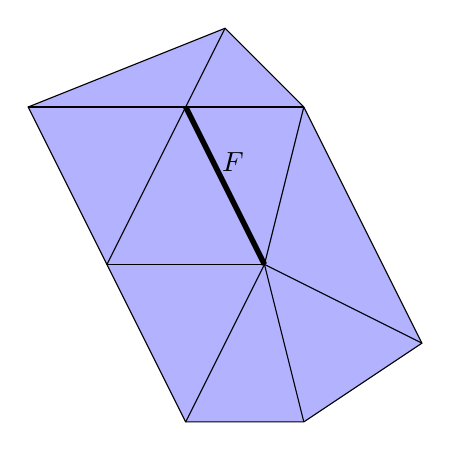
\begin{tikzpicture}
            % Define the coordinates
            \coordinate (A) at (0,0);
            \coordinate (B) at (2,0);
            \coordinate (C) at (1,2);
            \coordinate (D) at (2.5,2);
            \coordinate (F) at (1.5,3);
            \coordinate (E) at (-1,2);
            \coordinate (G) at (1,-2);
            \coordinate (H) at (2.5,-2);
            \coordinate (I) at (4,-1);

            \fill[blue!30] (A) -- (G)-- (H) -- (I)  -- (D) -- (F)-- (E)   -- cycle;

            % Draw the triangle
            \draw (A) -- (G)-- (H) -- (I)  -- (D) -- (F)-- (E)   -- cycle;
            \draw (A) -- (C);
            \draw (A) -- (B);
            \draw (G) -- (B);
            \draw (I) -- (B);
            \draw (F) -- (C);
            \draw (H) -- (B);
            \draw (D) -- (C);
            \draw (D) -- (B);
            \draw (E) -- (C);
            \draw[line width=2pt] (B) -- (C);
            \node at (1.6,1.3) {$F$};

        \end{tikzpicture}
    \end{minipage}\hfill

}}%
    \qquad
    \subfloat{{

    \begin{minipage}[b]{0.45\textwidth}
        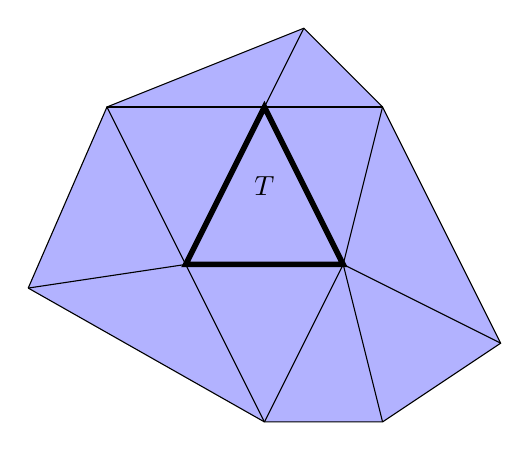
\begin{tikzpicture}
                    % Define the coordinates
        \coordinate (A) at (0,0);
        \coordinate (B) at (2,0);
        \coordinate (C) at (1,2);
        \coordinate (D) at (2.5,2);
        \coordinate (F) at (1.5,3);
        \coordinate (E) at (-1,2);
        \coordinate (G) at (1,-2);
        \coordinate (H) at (2.5,-2);
        \coordinate (I) at (4,-1);
        \coordinate (K) at (-2,-0.3);

        \fill[blue!30] (K) -- (G)-- (H) -- (I)  -- (D) -- (F)-- (E)   -- cycle;
        % \fill[red!30] (B) -- (C) -- (A);

        % Draw the triangle
        \draw (A) -- (G)-- (H) -- (I)  -- (D) -- (F)-- (E)   -- cycle;
        \draw (A) -- (C);
        \draw (A) -- (B);
        \draw (G) -- (B);
        \draw (I) -- (B);
        \draw (F) -- (C);
        \draw (H) -- (B);
        \draw (D) -- (C);
        \draw (D) -- (B);
        \draw (E) -- (C);
        \draw (K) -- (A);
        \draw (K) -- (G);
        \draw (K) -- (E);
        \draw[line width=2pt] (B) -- (C) -- (A) -- cycle;
        \node at (1.0,1.0) {$T$};

        \end{tikzpicture}
    \end{minipage}

    }}%
\caption{Illustration of the patch $\omega ( F) $ on the left-hand side and $\omega(T)$ on the right-hand side.}
    \label{fig:example_patch}%
\end{figure}

\begin{figure}[]
\begin{minipage}{.5\linewidth}
\centering
\subfloat[]{
    \label{fig:macroelements:a}
    \begin{tikzpicture}[scale=0.5]
        % Arbitrary triangle
        \coordinate (A1) at (0,0);
        \coordinate (B1) at (4,1);
        \coordinate (C1) at (1,3);
        \fill [blue!30] (A1) -- (B1) -- (C1) -- cycle;
        \draw (A1) -- (B1) -- (C1) -- cycle;

        % Centroid
        \coordinate (ai) at (barycentric cs:A1=1,B1=1,C1=1);
        \fill (ai) circle (2pt);
        \node[anchor=north east] at (ai) {$a_i$};

        % Reference triangle
        \coordinate (A2) at ($(A1) + (6, 0)$);
        \coordinate (B2) at ($(A2) + (0, 3)$);
        \coordinate (C2) at ($(A2) + (3, 0)$);
        \fill [red!30] (A2) -- (B2) -- (C2) -- cycle;
        \draw (A2) -- (B2) -- (C2) -- cycle;

        % Centroid of the reference triangle
        \coordinate (ahi) at (barycentric cs:A2=1,B2=1,C2=1);
        \fill (ahi) circle (2pt);
        \node[anchor=north west, xshift=-0.1cm, yshift=0.1cm] at (ahi) {$\hat{a}_{j( i)} $};

        \draw[->, thick, >=stealth] ($(ahi)+(0.2,+0.2)$) to[bend right] node[midway, above] {$\mathcal{G}_{A_i}$} ($(ai)+(0.2,+0.3)$);

    \end{tikzpicture}
}
\end{minipage}%
\begin{minipage}{.5\linewidth}
\centering
\subfloat[]{
    \label{fig:macroelements:b}
    \begin{tikzpicture}[scale=0.5]
    % Arbitrary square
    \coordinate (A1) at (0,0);
    \coordinate (B1) at (3,1);
    \coordinate (C1) at (4,4);
    \coordinate (D1) at (1,3);
    \fill[blue!30] (A1) -- (B1) -- (C1) -- (D1) -- cycle;
    \draw (A1) -- (B1) -- (C1) -- (D1) -- cycle;

    % Draw edge from D1 to B1
    \draw (D1) -- (B1);

    % Pick a point on the edge and label it as a_i
    \coordinate (a_i) at ($(D1)!.6!(B1)$);
    \fill (a_i) circle (2pt);
    \node[anchor=north] at (a_i) {$a_i$};

    % Reference equilateral triangle
    \coordinate (A2) at ($(A1) + (6, 0)$);
    \coordinate (B2) at ($(A2) + (2, 3.464)$); % 3.464 = 2 * sqrt(3)
    \coordinate (C2) at ($(A2) + (4, 0)$);
    \fill[red!30] (A2) -- (B2) -- (C2) -- cycle;
    \draw (A2) -- (B2) -- (C2) -- cycle;

    % Divide the equilateral triangle into two right triangles
    \coordinate (M) at ($(A2)!.5!(C2)$);
    \draw (B2) -- (M);

    % Pick a point on the shared edge and label it as ahat_i
    \coordinate (ahat_i) at ($(B2)!.7!(M)$);
    \fill (ahat_i) circle (2pt);
    \node[anchor=north west] at (ahat_i) {$\hat{a}_{j( i)} $};

    % Draw the mapping G_{A_i} from ahat_i to a_i
    \draw[->, thick, >=stealth] ($(ahat_i)+(0.2,0.2)$) to[bend right] node[midway, above] {$\mathcal{G}_{A_i}$} ($(a_i)+(0.2,0.2)$);
\end{tikzpicture}
}
\end{minipage}\par\medskip
\centering
\subfloat[]{
    \label{fig:macroelements:c}
 \begin{tikzpicture}[scale=0.5]

    % Central vertex a_i
    \coordinate (ah_i) at (0, 0);

    % Reference hexagon
    \foreach \angle in {0, 60, ..., 300} {
        \coordinate (A) at (\angle:2.5);
        \coordinate (B) at (\angle + 60:2.5);
        \fill[red!30] (ah_i) -- (A) -- (B) -- cycle;
        \draw (ah_i) -- (A) -- (B) -- cycle;
    }

    \fill (ah_i) circle (2pt);
    \node[anchor=east, yshift=0.25cm] at (ah_i) {$\hat{a}_{j( i) }$};

    \coordinate (A1) at (5, 0);
    \coordinate (B1) at (8, 0);
    \coordinate (C1) at (8, 3);
    \coordinate (D1) at (7, 4);
    \coordinate (E1) at (3.5, 4);
    \coordinate (F1) at (3, 2);
    \fill[blue!30] (A1) -- (B1) -- (C1) -- (D1) -- (E1) -- (F1) -- cycle;
    \draw (A1) -- (B1) -- (C1) -- (D1) -- (E1) -- (F1) -- cycle;

    \coordinate (ai) at (barycentric cs:A1=1,B1=1,C1=1,D1=1,E1=1,F1=1);
    % Draw lines from vertices to a_i
    \draw (A1) -- (ai);
    \draw (B1) -- (ai);
    \draw (C1) -- (ai);
    \draw (D1) -- (ai);
    \draw (E1) -- (ai);
    \draw (F1) -- (ai);
    % Centroid
    \fill (ai) circle (2pt);
    \node[anchor=south, yshift=0.2cm] at (ai) {$a_i$};

    \draw[->, thick, >=stealth] ($(ah_i)+(0.2,- 0.2)$) to[bend right] node[midway, above, yshift=0.1cm] {$\mathcal{G}_{A_i}$} ($(ai)+(-0.2,-0.2)$);

\end{tikzpicture}
}

\caption{Illustration of the different cases when mapping from the reference macroelement $\widehat{A}_{j( i) }$  to the domain $A_{i}$,  $\mathcal{G} _{A_{i}}: \widehat{A}_{j( i) } \to A_{i}$. Here we have defined $\hat{a}_{j(i)} \in
    \widehat{A}_{j(i)}$ s.t. $\mathcal{G}_{A_{i}} ( \hat{a}_{j( i) }) = a_i$. }

\label{fig:macroelements}
\end{figure}


 Let the set  $\left\{ a_{i}\right\}_{i\in N}$ be all Lagrange nodes on the mesh $\mathcal{T}_{h}$. Associated with each node $a_{i}$ we denote the macroelement $A_{i}$ to consist of all elements containing $a_{i}$. Let $n_{cf}$ be the number of configurations for the macroelement, then we define the index $j:
\left\{ 1,\ldots,N \right\} \to \left\{ 1, \ldots, n_{cf} \right\}  $ s.t. $j( i) $ is the index associated with the reference configuration $\widehat{A}_{j(i) }$ for corresponding macroelement $A_{i}$.
Let us define a $C^{0}$-diffeomorphism $\mathcal{G}_{A_{i}}:
\widehat{A}_{j( i) } \to A_{i}$ on the reference macroelements such that for all $\hat{T} \in \widehat{A}_{j( i) } $ is the restriction $\mathcal{G} _{A_{i}}|_{ \hat{T} }$ affine. For an illustration of the reference
macroelement $\widehat{A}_{j( i) }$ and how it related to $a_{i}$ , see
Figure \ref{fig:macroelements}.

The Cléments interpolation operator $C_{h}$ is the $L^2$-projection onto the macroelements. That is, given
a reference macroelement $\widehat{A}_{j( i) }$ and a function $\hat{v} \in L^{1}( \widehat{A}_{j( i) })  $, then $\widehat{C}_{j( i) } \hat{v}$  is the unique polynomial in $\mathcal{P}^{k} ( \widehat{A}_{j( i) })  $ s.t. \[
\int_{  \widehat{A}_{j( i) }}^{} ( \widehat{C}_{j( i) } \hat{v} - \hat{v}) p \ dx  = 0 \quad  \forall p \in \mathcal{P}^{k} ( \widehat{A}_{j( i) })
\]
Finally, the Cléments interpolator is defined as the mapping $C_{h} : L^{1}( \Omega )  \to \mathcal{P} ^{k}_{c}(\mathcal{T}_{h}   ) $ such that
\[
C_{h} v = \sum_{i=1}^{N} \widehat{C}_{j( i) } ( v (\mathcal{G} _{A_{i}}) (\mathcal{G}^{-1}_{A_{i}}(a_{i})) )\phi _{i},
\]
where $\phi _{i}$ is the corresponding polynomial basis associated with the node $a_{i}$.

Recall the general Sobolev norm notation,
\[
\| u \|_{ m,p,T }^{  } = \left( \sum_{ \left\lvert \alpha  \right\rvert \le m}^{} \int_{T}^{}  \left\lvert  \partial ^{\alpha } u \right\rvert^{p} dx   \right)^{\frac{1}{2}}
\]
where we use the convenient notation $\| u \|_{L^2(T) }^{  } = \| u \|_{ T  }^{  } = \| u \|_{ 0,2,T  }^{  } $ and similarly $\| u \|_{ H^r( T )  }^{  } = \| u \|_{ r,T  }^{  } = \| u \|_{ r,2,T  }^{  }  $.


Finally, we have the following lemma

\begin{lemma}
    \label{lemma:clements}

We define the Clement interpolation as the projection
$C_{h}: H^{m} \left( \Omega  \right) \mapsto V_{h}$, where $V_{h}$ has the order $k$. Then does the following stability estimate hold,
\[
 \| C_{h} v \|_{H^{m}\left( \Omega  \right)   }^{  } \lesssim \| v \|_{ H^{m}\left( \Omega  \right)  }^{  } \quad \forall v \in H^{m}\left( \Omega  \right),
\]
and if the following conditions for an parameter $l$ is satisfied, it exists error estimates s.t.,
\[
    \begin{split}
      m\le l \le k+1  \implies \| v - C_{h} v \|_{ m,p,T   }^{  }  &  \lesssim h^{l-m}_{T} \| v \|_{l,p,\omega \left( T \right)  }^{  } \quad  \forall T \in \mathcal{T} _{h}, \forall v \in H^{l}( \omega \left( T \right)
      ), \\
      m +\frac{1}{2}\le l \le k+1  \implies \| v - C_{h} v \|_{ m,p,F }^{  } & \lesssim h^{l-m- \frac{1}{2}}_{T} \| v \|_{l,p,\omega \left( F \right)  }^{  } \quad  \forall \partial T \in \mathcal{T} _{h}, \forall v \in H^{l}( \omega \left( F
      \right)).
    \end{split}
\]

\end{lemma}


\begin{corollary}
    \label{cor:celement_apriori}
    Let $0 \le l \le k+1$ and let $0\le m \le \min_{} ( 1,l )$.
    Given Lemma \ref{lemma:clements}  then there exists an $C > 0$ s.t.
    \[
    \inf_{v_{h} \in \mathcal{P} ^{k}_{c}( \Omega ) } \| v - v_{h} \|_{  m,p,\Omega }^{  } \le C h^{l-m}  \| v \|_{ l,p,\Omega  }^{  }    \forall v \in W_{l,p}( \Omega ).
    \]
\end{corollary}
This result is very useful since it is now sufficient to show that a priori estimates holds to prove convergence rate. For further detailed information about the Cléments interpolation, please investigate \cite[Chapter 1.6]{ern04}.
We will use these estimates to compute convergence rate given that Ceas' Lemma holds.

\subsection{Ceas Lemma}%
\label{sub:ceas_lemma}


Assume that we have a discrete bilinear form $a_{h}: X_{h}\times X_{h} \to \mathbb{R} $ and let $X _{h} \subseteq  X $ be the discrete polynomial space. We transition the problem to find a solution, $u_{h} \in  \mathcal{V}_{h}$, so it holds that $a\left( u_{h},v_{h} \right)  = l\left( v_{h} \right) \ \  \forall v_{h} \in X _{h} $.
Since the method is conform, i.e., $X _{h} \subseteq  X $, does it exists a exact solution, $u \in  \mathcal{V}$, such that \(
a \left( u, v_{h} \right)  = l\left( v_{h} \right)  \ \  \forall v_{h} \in  X _{h}.
\)
Furthermore, the problem is said to be strongly consistent since it fulfills the Galerkin orthogonality property, that is $ a\left( u -u_{h} , v_{h} \right)  =0$. Thus, if $u_{h},v_{h} \in  X _{h}$, then
\begin{equation}
\label{eq:cealemma_proof}
    \begin{split}
\alpha \| u -u_{h} \|_{ X  }^{ 2 } & \le  a\left( u - u_{h}, u - u_{h}  \right)    \\
&= a\left( u - u_{h}, u -v_{h} \right) - a\left( u -u_{h}, v_{h} - u_{h} \right)  \\
 &  \le  M \| u - u_{h} \|_{ X  }^{  }  \| u - v_{h} \|_{ X  }^{  }
    \end{split}
.\end{equation}
Hence, we now have the so-called Ceas lemma, \[
\| u - u_{h} \|_{ X  }^{  }  \lesssim  \inf_{v_{h} \in X_{h} } \|  v_{h} - u \|_{X  }^{  }.
\]
A useful property is that for a conformal numerical method to converge can we now simply require \[
\lim_{h \to 0}  \inf_{v_{h} \in  X_{h}}  \| v - v_{h} \|_{ X  }^{  } = 0 \quad  \forall v \in X.
\]
In that case will $\| u - u_{h} \|_{ X  }^{  }  \to  0$, $h \to  0$. Hence, if this requirement is fulfilled, the numerical methods will converge to a unique solution.
For more information, see \cite[pp. 66]{quartdiff}.

In combination with Corollary \ref{cor:celement_apriori}, is Ceas lemma very handy to construct a priori estimates. However, Ceas lemma as it stands does assume conform methods $X_{h} \subset X$, hence, we must be cautious for broken Sobolev spaces.
 



